%%%%%%%%%%%%%%%%%%%%%%%%%%%%%%%%%%%%%%%%%%%%%%%%%%%%%%%%%%%%%%%%%%%%%%%%%%%%%%%%
%
% Template license:
% CC BY-NC-SA 3.0 (http://creativecommons.org/licenses/by-nc-sa/3.0/)
%
%%%%%%%%%%%%%%%%%%%%%%%%%%%%%%%%%%%%%%%%%%%%%%%%%%%%%%%%%%%%%%%%%%%%%%%%%%%%%%%%

%----------------------------------------------------------------------------------------
%	PACKAGES AND OTHER DOCUMENT CONFIGURATIONS
%----------------------------------------------------------------------------------------

\documentclass[
11pt, % The default document font size, options: 10pt, 11pt, 12pt
%oneside, % Two side (alternating margins) for binding by default, uncomment to switch to one side
%chapterinoneline,% Have the chapter title next to the number in one single line
spanish,
singlespacing, % Single line spacing, alternatives: onehalfspacing or doublespacing
%draft, % Uncomment to enable draft mode (no pictures, no links, overfull hboxes indicated)
%nolistspacing, % If the document is onehalfspacing or doublespacing, uncomment this to set spacing in lists to single
%liststotoc, % Uncomment to add the list of figures/tables/etc to the table of contents
%toctotoc, % Uncomment to add the main table of contents to the table of contents
parskip, % Uncomment to add space between paragraphs
%codirector, % Uncomment to add a codirector to the title page
headsepline, % Uncomment to get a line under the header
]{MastersDoctoralThesis} % The class file specifying the document structure



%----------------------------------------------------------------------------------------
%	INFORMACIÓN DE LA MEMORIA
%----------------------------------------------------------------------------------------

\thesistitle{Sistema de monitoreo para planta de acopio de cereales} % El títulos de la memoria, se usa en la carátula y se puede usar el cualquier lugar del documento con el comando \ttitle

% Nombre del posgrado, se usa en la carátula y se puede usar el cualquier lugar del documento con el comando \degreename
\posgrado{Carrera de Especialización en Internet de las Cosas} 
%\posgrado{Carrera de Especialización en Internet de las Cosas} 
%\posgrado{Carrera de Especialización en Intelegencia Artificial}
%\posgrado{Maestría en Sistemas Embebidos} 
%\posgrado{Maestría en Internet de las cosas}

\author{Ing. Lucas Eduardo Olmedo} % Tu nombre, se usa en la carátula y se puede usar el cualquier lugar del documento con el comando \authorname

\director{Esp. Ing. Marcelo Castello (UTN-FRRO)} % El nombre del director, se usa en la carátula y se puede usar el cualquier lugar del documento con el comando \dirname
\codirector{Nombre del codirector (pertenencia)} % El nombre del codirector si lo hubiera, se usa en la carátula y se puede usar el cualquier lugar del documento con el comando \codirname.  Para activar este campo se debe descomentar la opción "codirector" en el comando \documentclass, línea 23.

\juradoUNO{Nombre del jurado 1 (pertenencia)} % Nombre y pertenencia del un jurado se usa en la carátula y se puede usar el cualquier lugar del documento con el comando \jur1name
\juradoDOS{Nombre del jurado 2 (pertenencia)} % Nombre y pertenencia del un jurado se usa en la carátula y se puede usar el cualquier lugar del documento con el comando \jur2name
\juradoTRES{Nombre del jurado 3 (pertenencia)} % Nombre y pertenencia del un jurado se usa en la carátula y se puede usar el cualquier lugar del documento con el comando \jur3name

%\ciudad{Ciudad Autónoma de Buenos Aires}
\ciudad{ciudad de Córdoba}

\fechaINICIO{marzo de 2023}
\fechaFINAL{marzo de 2024}


\keywords{Internet de las cosas, FIUBA} % Keywords for your thesis, print it elsewhere with \keywordnames


\begin{document}


\frontmatter % Use roman page numbering style (i, ii, iii, iv...) for the pre-content pages

\pagestyle{plain} % Default to the plain heading style until the thesis style is called for the body content


%----------------------------------------------------------------------------------------
%	RESUMEN - ABSTRACT 
%----------------------------------------------------------------------------------------

\begin{abstract}
\addchaptertocentry{\abstractname} % Add the abstract to the table of contents
%
%The Thesis Abstract is written here (and usually kept to just this page). The page is kept centered vertically so can expand into the blank space above the title too\ldots
\centering

En la presente memoria se describe el diseño, desarrollo e implementación de un
sistema de monitoreo para una planta de acopio de cereales. Este es un proyecto personal que surge de la necesidad de reducir tiempos y optimizar costos en la empresa de un posible cliente. 

En el trabajo se aplicaron conocimientos de desarrollo de software, ciberseguridad, protocolos de comunicación e infraestructura para el almacenamiento, procesamiento y visualización de los datos de interés. 

\end{abstract}

%----------------------------------------------------------------------------------------
%	CONTENIDO DE LA MEMORIA  - AGRADECIMIENTOS
%----------------------------------------------------------------------------------------

\begin{acknowledgements}
%\addchaptertocentry{\acknowledgementname} % Descomentando esta línea se puede agregar los agradecimientos al índice
\vspace{1.5cm}

Esta sección es para agradecimientos personales y es totalmente \textbf{OPCIONAL}.  

\end{acknowledgements}

%----------------------------------------------------------------------------------------
%	LISTA DE CONTENIDOS/FIGURAS/TABLAS
%----------------------------------------------------------------------------------------

\tableofcontents % Prints the main table of contents

\listoffigures % Prints the list of figures

\listoftables % Prints the list of tables


%----------------------------------------------------------------------------------------
%	CONTENIDO DE LA MEMORIA  - DEDICATORIA
%----------------------------------------------------------------------------------------

%\dedicatory{\textbf{Dedicado a... [OPCIONAL]}}  % escribir acá si se desea una dedicatoria

%----------------------------------------------------------------------------------------
%	CONTENIDO DE LA MEMORIA  - CAPÍTULOS
%----------------------------------------------------------------------------------------

\mainmatter % Begin numeric (1,2,3...) page numbering

\pagestyle{thesis} % Return the page headers back to the "thesis" style

% Incluir los capítulos como archivos separados desde la carpeta Chapters

% Chapter 1

\chapter{Introducción general} % Main chapter title

\label{Chapter1} % For referencing the chapter elsewhere, use \ref{Chapter1} 
\label{IntroGeneral}

%----------------------------------------------------------------------------------------

% Define some commands to keep the formatting separated from the content 
\newcommand{\keyword}[1]{\textbf{#1}}
\newcommand{\tabhead}[1]{\textbf{#1}}
\newcommand{\code}[1]{\texttt{#1}}
\newcommand{\file}[1]{\texttt{\bfseries#1}}
\newcommand{\option}[1]{\texttt{\itshape#1}}
\newcommand{\grados}{$^{\circ}$}

%----------------------------------------------------------------------------------------

En este capítulo se presenta una breve introducción sobre el acopio de cereales y la necesidad de monitorizarlo, soluciones existentes, motivos por los cuales se seleccionó el tema, objetivos y alcance del trabajo. 
%----------------------------------------------------------------------------------------
\section{Descripción de la problemática}

\subsection{Plantas de acopio}

Las plantas de acopio de cereales son depósitos donde se almacenan las semillas luego de ser cosechadas en el campo, a la espera de ser despachadas a su destino final. Estas plantas están compuestas por uno o más silos como puede observarse en la figura \ref{fig:planta}

\begin{figure}[htbp]
	\centering
	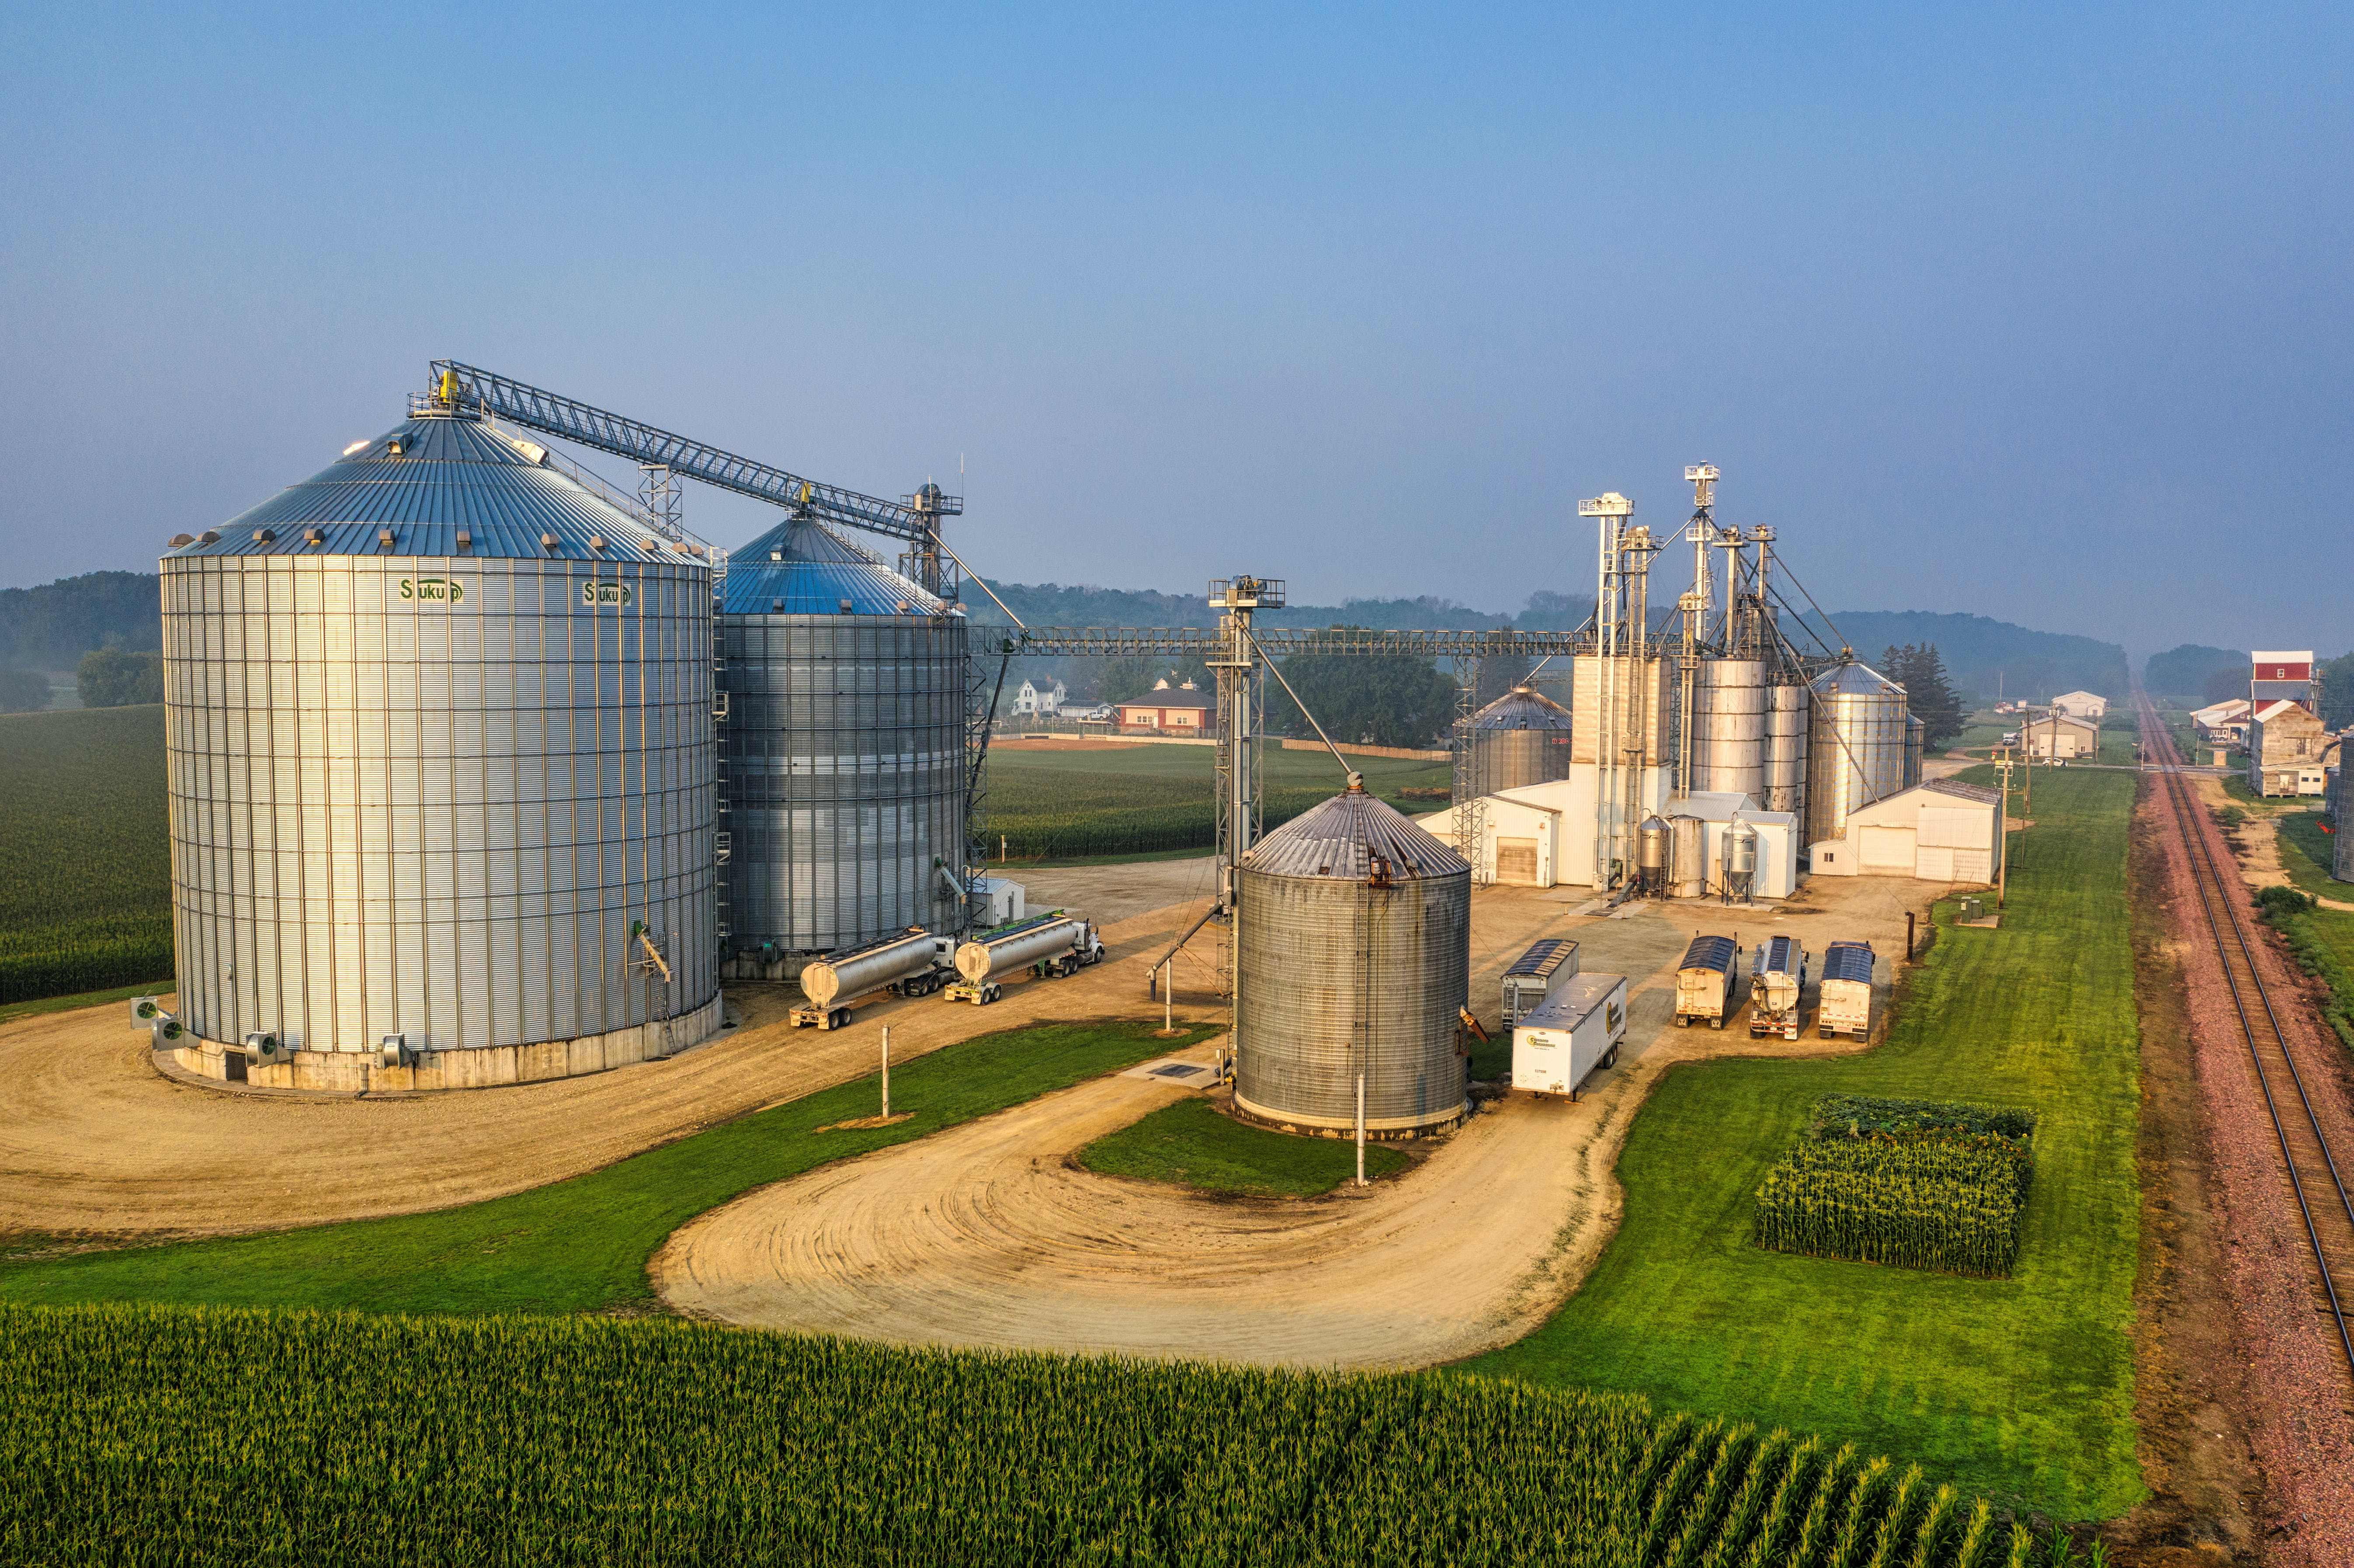
\includegraphics[width=.5\textwidth]{./Figures/PlantaAcopio.jpg}
	\caption{Planta de acopio de cereales.\protect\footnotemark}
	\label{fig:planta}
\end{figure}
\footnotetext{Imagen tomada de \url{https://www.pexels.com/es-es/}}

Los silos son construcciones para almacenar granos y otros materiales a granel. Se pueden fabricar con diferentes materiales y diseños. \citep{WEBSITE:6}
%https://es.wikipedia.org/wiki/Silo

Los acopios de cereales proveen a los productores agropecuarios un espacio de almacenamiento para las semillas cosechadas. El objetivo es preservar el cereal en condiciones óptimas durante un periodo de tiempo prolongado para luego poder comercializarlo y maximizar la calidad de los productos que derivan de ellos. \citep{ARTICLE:1}

\subsection{Condiciones de almacenamiento de granos}

Para reducir las pérdidas de calidad y de inocuidad debe comprenderse que los granos tienen dos enemigos
principales: los hongos y los insectos. En consecuencia, todos los esfuerzos que se realicen durante la poscosecha deben estar claramente orientados a prevenir el desarrollo de estos organismos perjudiciales para el grano. \citep{ARTICLE:1}

Para un almacenaje seguro, evitando hongos e insectos, es necesario que dentro del silo se registre baja temperatura y humedad. 

Conocer el contenido de humedad de los granos es imprescindible para una adecuada conservación de las semillas durante la poscosecha, pues la humedad determinará en gran medida el período durante el cual el grano puede ser almacenado sin que se deteriore su calidad. Por lo tanto, conocer la humedad será fundamental para tomar la mejor decisión en cuanto a secar el grano, acondicionarlo o almacenarlo directamente.

La humedad de almacenamiento seguro es aquella que evita el desarrollo de hongos. Esta es afectada por la humedad ambiente.

El tiempo de almacenamiento seguro es el período máximo que puede ser almacenado un grano a determinadas condiciones de humedad y temperatura, sin perder su calidad o propiedades.
Este es afectado por tres factores:

\begin{itemize}
\item La humedad con que es almacenado el grano, la cual favorece fundamentalmente el desarrollo de los hongos.
\item La temperatura. Cuanto mayor es, más rápido es el deterioro y favorece la propagación a los insectos.
\item El porcentaje de grano dañado mecánicamente. Este es más susceptible al ataque de hongos y de insectos.
\end{itemize}

Como se puede observar en la figura \ref{fig:tempHum}, la forma óptima de conservar los cereales es mantener baja temperatura y humedad.

\begin{figure}[htbp]
	\centering
	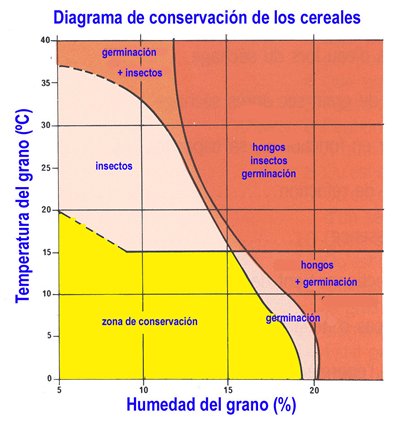
\includegraphics[width=.5\textwidth]{./Figures/DiagramaDeConservacionGranos.png}
	\caption{Diagrama conservación de los cereales.\protect\footnotemark}
	\label{fig:tempHum}
\end{figure}
\footnotetext{Imagen tomada de \url{https://www.mapa.gob.es/es/ministerio/servicios/informacion/plataforma-de-conocimiento-para-el-medio-rural-y-pesquero/observatorio-de-tecnologias-probadas/maquinaria-agricola/secado-grano.aspx}}

Las condiciones que perjudican la calidad del grano se debe monitorear periódicamente para detectar cuanto antes potenciales inconvenientes, como la combustión espontánea, y tomar acciones preventivas evitando el deterioro de las semillas. \citep{WEBSITE:5}

%----------------------------------------------------------------------------------------
\section{Estado del arte}

Si bien existen soluciones similares, pocas se encuentran en el país, lo cual implica que los costos y mantenimiento sean elevados. 

El objetivo del trabajo es crear un prototipo de monitoreo de temperatura y humedad en una planta de acopio de cereales. Luego de ello, como mejora a futuro, se pretende migrar a una solución IoT integral donde se incluyan otros tipos de sensores que faciliten la logística y seguridad en la planta. 

En la tabla \ref{tab:peces} se observan algunas alternativas para monitoreo de parámetros en almacenamiento de cereales.

\begin{table}[h]
	\centering
	\caption[]{Soluciones existentes para monitoreo en almacenamiento de cereales}
	\begin{tabular}{l c c c}    
		\toprule
		\textbf{Empresa} 	 & \textbf{Temperatura} 		& \textbf{Humedad} & \textbf{Referencia} \\
		\midrule
		  OPI & sí	& sí  & \citep{WEBSITE:4}\\		
		Avann Technologies	 & sí	& sí & \citep{WEBSITE:3}\\
		Measure Instruments	 & sí	& no & \citep{WEBSITE:1} \\
            Tornum	 & sí	& sí  & \citep{WEBSITE:2}\\
		\bottomrule
		\hline
	\end{tabular}
	\label{tab:peces}
\end{table}

En resumen, se encuentran soluciones comerciales que permiten el monitoreo de temperatura y humedad. Sin embargo, el objetivo de este trabajo es lograr consolidar los conocimientos adquiridos en la especialidad y generar una solución incremental que permita llegar a la automatización total de una planta de acopio de cereales con un costo accesible. 

%----------------------------------------------------------------------------------------
\section{Motivación}
Una empresa o cooperativa dedicada al almacenamiento de granos tiene uno o más depósitos distribuidos y para controlar el estado de almacenamiento de sus productos necesita enviar operarios a las diferentes plantas. Dada esta situación, se implementó un sistema de monitoreo IoT para optimizar tiempos y costos.

Al comenzar a buscar posibles temas para este trabajo, surgió el contacto con un posible cliente que necesita una solución integral de IoT para su planta de acopio, por este motivo se implementa un prototipo que luego irá evolucionando e integrando soluciones a diferentes problemas. 

%----------------------------------------------------------------------------------------
\section{Alcance y objetivos}

El propósito de este trabajo fue implementar el prototipo de un sistema de monitoreo para plantas de acopio de cereales, con el objetivo de reafirmar los conocimientos adquiridos en la especialización de internet de las cosas y poder implementarlo a futuro en campo. 

Esta implementación será la base de futuros desarrollos donde se planifica integrar diferentes tipos de sensores y adaptar el proyecto a las necesidades de algunos clientes.  

El alcance del trabajo incluyó:
\begin{itemize}
\item Un prototipo funcional.
\item Un nodo que simula datos obtenidos y los transmite a la nube.
\item Selección del protocolo para transmisión de datos.
\item Desarrollo / selección de \textit{backend} del sistema que procesa y almacena los datos recibidos.
\item Presentación de datos.
\end{itemize}

El presente trabajo no incluye:
\begin{itemize}
    \item La puesta en marcha del producto en las instalaciones de una planta de almacenamiento.
    \item La lectura de datos en sensores reales desde los nodos.
\end{itemize}

%----------------------------------------------------------------------------------------



%\chapter{Introducción específica} % Main chapter title

\label{Chapter2}

%----------------------------------------------------------------------------------------
%	SECTION 1
%----------------------------------------------------------------------------------------
Todos los capítulos deben comenzar con un breve párrafo introductorio que indique cuál es el contenido que se encontrará al leerlo.  La redacción sobre el contenido de la memoria debe hacerse en presente y todo lo referido al proyecto en pasado, siempre de modo impersonal.

\section{Estilo y convenciones}
\label{sec:ejemplo}

\subsection{Uso de mayúscula inicial para los título de secciones}

Si en el texto se hace alusión a diferentes partes del trabajo referirse a ellas como capítulo, sección o subsección según corresponda. Por ejemplo: ``En el capítulo \ref{Chapter1} se explica tal cosa'', o ``En la sección \ref{sec:ejemplo} se presenta lo que sea'', o ``En la subsección \ref{subsec:ejemplo} se discute otra cosa''.

Cuando se quiere poner una lista tabulada, se hace así:

\begin{itemize}
	\item Este es el primer elemento de la lista.
	\item Este es el segundo elemento de la lista.
\end{itemize}

Notar el uso de las mayúsculas y el punto al final de cada elemento.

Si se desea poner una lista numerada el formato es este:

\begin{enumerate}
	\item Este es el primer elemento de la lista.
	\item Este es el segundo elemento de la lista.
\end{enumerate}

Notar el uso de las mayúsculas y el punto al final de cada elemento.

\subsection{Este es el título de una subsección}
\label{subsec:ejemplo}

Se recomienda no utilizar \textbf{texto en negritas} en ningún párrafo, ni tampoco texto \underline{subrayado}. En cambio sí se debe utilizar \textit{texto en itálicas} para palabras en un idioma extranjero, al menos la primera vez que aparecen en el texto. En el caso de palabras que estamos inventando se deben utilizar ``comillas'', así como también para citas textuales. Por ejemplo, un \textit{digital filter} es una especie de ``selector'' que permite separar ciertos componentes armónicos en particular.

La escritura debe ser impersonal. Por ejemplo, no utilizar ``el diseño del firmware lo hice de acuerdo con tal principio'', sino ``el firmware fue diseñado utilizando tal principio''. 

El trabajo es algo que al momento de escribir la memoria se supone que ya está concluido, entonces todo lo que se refiera a hacer el trabajo se narra en tiempo pasado, porque es algo que ya ocurrió. Por ejemplo, "se diseñó el firmware empleando la técnica de test driven development".

En cambio, la memoria es algo que está vivo cada vez que el lector la lee. Por eso transcurre siempre en tiempo presente, como por ejemplo:

``En el presente capítulo se da una visión global sobre las distintas pruebas realizadas y los resultados obtenidos. Se explica el modo en que fueron llevados a cabo los test unitarios y las pruebas del sistema''.

Se recomienda no utilizar una sección de glosario sino colocar la descripción de las abreviaturas como parte del mismo cuerpo del texto. Por ejemplo, RTOS (\textit{Real Time Operating System}, Sistema Operativo de Tiempo Real) o en caso de considerarlo apropiado mediante notas a pie de página.

Si se desea indicar alguna página web utilizar el siguiente formato de referencias bibliográficas, dónde las referencias se detallan en la sección de bibliografía de la memoria, utilizado el formato establecido por IEEE en \citep{IEEE:citation}. Por ejemplo, ``el presente trabajo se basa en la plataforma EDU-CIAA-NXP \citep{CIAA}, la cual...''.

\subsection{Figuras} 

Al insertar figuras en la memoria se deben considerar determinadas pautas. Para empezar, usar siempre tipografía claramente legible. Luego, tener claro que \textbf{es incorrecto} escribir por ejemplo esto: ``El diseño elegido es un cuadrado, como se ve en la siguiente figura:''

\begin{figure}[h]
\centering
\includegraphics[scale=.45]{./Figures/cuadradoAzul.png}
\end{figure}

La forma correcta de utilizar una figura es con referencias cruzadas, por ejemplo: ``Se eligió utilizar un cuadrado azul para el logo, como puede observarse en la figura \ref{fig:cuadradoAzul}''.

\begin{figure}[ht]
	\centering
	\includegraphics[scale=.45]{./Figures/cuadradoAzul.png}
	\caption{Ilustración del cuadrado azul que se eligió para el diseño del logo.}
	\label{fig:cuadradoAzul}
\end{figure}

El texto de las figuras debe estar siempre en español, excepto que se decida reproducir una figura original tomada de alguna referencia. En ese caso la referencia de la cual se tomó la figura debe ser indicada en el epígrafe de la figura e incluida como una nota al pie, como se ilustra en la figura \ref{fig:palabraIngles}.

\begin{figure}[htpb]
	\centering
	\includegraphics[scale=.3]{./Figures/word.jpeg}
	\caption{Imagen tomada de la página oficial del procesador\protect\footnotemark.}
	\label{fig:palabraIngles}
\end{figure}

\footnotetext{Imagen tomada de \url{https://goo.gl/images/i7C70w}}

La figura y el epígrafe deben conformar una unidad cuyo significado principal pueda ser comprendido por el lector sin necesidad de leer el cuerpo central de la memoria. Para eso es necesario que el epígrafe sea todo lo detallado que corresponda y si en la figura se utilizan abreviaturas entonces aclarar su significado en el epígrafe o en la misma figura.



\begin{figure}[ht]
	\centering
	\includegraphics[scale=.37]{./Figures/questionMark.png}
	\caption{¿Por qué de pronto aparece esta figura?}
	\label{fig:questionMark}
\end{figure}

Nunca colocar una figura en el documento antes de hacer la primera referencia a ella, como se ilustra con la figura \ref{fig:questionMark}, porque sino el lector no comprenderá por qué de pronto aparece la figura en el documento, lo que distraerá su atención.

Otra posibilidad es utilizar el entorno \textit{subfigure} para incluir más de una figura, como se puede ver en la figura \ref{fig:three graphs}. Notar que se pueden referenciar también las figuras internas individualmente de esta manera: \ref{fig:1de3}, \ref{fig:2de3} y \ref{fig:3de3}.
 
\begin{figure}[!htpb]
     \centering
     \begin{subfigure}[b]{0.3\textwidth}
         \centering
         \includegraphics[width=.65\textwidth]{./Figures/questionMark}
         \caption{Un caption.}
         \label{fig:1de3}
     \end{subfigure}
     \hfill
     \begin{subfigure}[b]{0.3\textwidth}
         \centering
         \includegraphics[width=.65\textwidth]{./Figures/questionMark}
         \caption{Otro.}
         \label{fig:2de3}
     \end{subfigure}
     \hfill
     \begin{subfigure}[b]{0.3\textwidth}
         \centering
         \includegraphics[width=.65\textwidth]{./Figures/questionMark}
         \caption{Y otro más.}
         \label{fig:3de3}
     \end{subfigure}
        \caption{Tres gráficos simples}
        \label{fig:three graphs}
\end{figure}

El código para generar las imágenes se encuentra disponible para su reutilización en el archivo \file{Chapter2.tex}.

\subsection{Tablas}

Para las tablas utilizar el mismo formato que para las figuras, sólo que el epígrafe se debe colocar arriba de la tabla, como se ilustra en la tabla \ref{tab:peces}. Observar que sólo algunas filas van con líneas visibles y notar el uso de las negritas para los encabezados.  La referencia se logra utilizando el comando \verb|\ref{<label>}| donde label debe estar definida dentro del entorno de la tabla.

\begin{verbatim}
\begin{table}[h]
	\centering
	\caption[caption corto]{caption largo más descriptivo}
	\begin{tabular}{l c c}    
		\toprule
		\textbf{Especie}     & \textbf{Tamaño} & \textbf{Valor}\\
		\midrule
		Amphiprion Ocellaris & 10 cm           & \$ 6.000 \\		
		Hepatus Blue Tang    & 15 cm           & \$ 7.000 \\
		Zebrasoma Xanthurus  & 12 cm           & \$ 6.800 \\
		\bottomrule
		\hline
	\end{tabular}
	\label{tab:peces}
\end{table}
\end{verbatim}


\begin{table}[h]
	\centering
	\caption[caption corto]{caption largo más descriptivo}
	\begin{tabular}{l c c}    
		\toprule
		\textbf{Especie} 	 & \textbf{Tamaño} 		& \textbf{Valor}  \\
		\midrule
		Amphiprion Ocellaris & 10 cm 				& \$ 6.000 \\		
		Hepatus Blue Tang	 & 15 cm				& \$ 7.000 \\
		Zebrasoma Xanthurus	 & 12 cm				& \$ 6.800 \\
		\bottomrule
		\hline
	\end{tabular}
	\label{tab:peces}
\end{table}

En cada capítulo se debe reiniciar el número de conteo de las figuras y las tablas, por ejemplo, figura 2.1 o tabla 2.1, pero no se debe reiniciar el conteo en cada sección. Por suerte la plantilla se encarga de esto por nosotros.

\subsection{Ecuaciones}
\label{sec:Ecuaciones}

Al insertar ecuaciones en la memoria dentro de un entorno \textit{equation}, éstas se numeran en forma automática  y se pueden referir al igual que como se hace con las figuras y tablas, por ejemplo ver la ecuación \ref{eq:metric}.

\begin{equation}
	\label{eq:metric}
	ds^2 = c^2 dt^2 \left( \frac{d\sigma^2}{1-k\sigma^2} + \sigma^2\left[ d\theta^2 + \sin^2\theta d\phi^2 \right] \right)
\end{equation}
                                                        
Es importante tener presente que si bien las ecuaciones pueden ser referidas por su número, también es correcto utilizar los dos puntos, como por ejemplo ``la expresión matemática que describe este comportamiento es la siguiente:''

\begin{equation}
	\label{eq:schrodinger}
	\frac{\hbar^2}{2m}\nabla^2\Psi + V(\mathbf{r})\Psi = -i\hbar \frac{\partial\Psi}{\partial t}
\end{equation}

Para generar la ecuación \ref{eq:metric} se utilizó el siguiente código:

\begin{verbatim}
\begin{equation}
	\label{eq:metric}
	ds^2 = c^2 dt^2 \left( \frac{d\sigma^2}{1-k\sigma^2} + 
	\sigma^2\left[ d\theta^2 + 
	\sin^2\theta d\phi^2 \right] \right)
\end{equation}
\end{verbatim}

Y para la ecuación \ref{eq:schrodinger}:

\begin{verbatim}
\begin{equation}
	\label{eq:schrodinger}
	\frac{\hbar^2}{2m}\nabla^2\Psi + V(\mathbf{r})\Psi = 
	-i\hbar \frac{\partial\Psi}{\partial t}
\end{equation}

\end{verbatim} 
%\include{Chapters/Chapter3}
%\include{Chapters/Chapter4} 
%\include{Chapters/Chapter5} 

%----------------------------------------------------------------------------------------
%	CONTENIDO DE LA MEMORIA  - APÉNDICES
%----------------------------------------------------------------------------------------

\appendix % indicativo para indicarle a LaTeX los siguientes "capítulos" son apéndices

% Incluir los apéndices de la memoria como archivos separadas desde la carpeta Appendices
% Descomentar las líneas a medida que se escriben los apéndices

%\include{Appendices/AppendixA}
%\include{Appendices/AppendixB}
%\include{Appendices/AppendixC}

%----------------------------------------------------------------------------------------
%	BIBLIOGRAPHY
%----------------------------------------------------------------------------------------

\Urlmuskip=0mu plus 1mu\relax
\raggedright
\printbibliography[heading=bibintoc]

%----------------------------------------------------------------------------------------

\end{document}  
